In den nächsten Unterkapiteln soll zunächst ein historischer Überblick über die Programmiersprache JavaScript gegeben werden. Im Anschluss wird auf die Bedeutung und Nutzung von JavaScript eingegangen. 
\newline

\subsubsection{Historie}
Ihren Ursprung findet die Programmiersprache JavaScript im Jahr 1995, als Brendan Eich, ein damaliger Ingenieur des US-amerikanischen Software-Unternehmens „Netscape Communications Corporation“, innerhalb von zehn Tagen diese Sprache für den Browser „Netscape Navigator“ entwickelt hat \cite{JS1}. Das Ziel dabei war es, eine Skriptsprache zu entwickeln, die es Entwicklern möglich machen sollte, auf ihren Webseiten Skripte umzusetzen. Zunächst noch unter dem Namen Mocha und LiveScript änderte sich der Name zu JavaScript aufgrund der Kooperation von Netscape und Sun, der Firma hinter der Programmiersprache Java, und Marketinggründen. Netscape wollte von der damaligen Popularität von Java profitieren \cite{JS1.05}. 
\newline
\noindent
Netscape’s Veröffentlichung des Netscape Navigator 2.0, der erste Browser der JavaScript unterstützte, brachte Microsoft dazu, Netscape als ernstzunehmenden Konkurrenten zu sehen. 
Microsoft antwortete im August 1995 mit der Veröffentlichung des ersten Internet Explorer zusammen mit der Skriptsprache JScript, die einen Dialekt der Sprache JavaScript darstellt. Dies ist ferner als der Beginn der „Browserkriege“ bekannt\cite{JS1.06}.
\newline
\noindent
Im Jahre 1997 reichte Netscape JavaScript bei der European Computer Manufacturers Association (kurz ECMA), einer privaten, internationalen Normungsorganisation zur Normung von Informations- und Kommunikationssystemen und Unterhaltungselektronik, ein. Das Ziel war es, von der ECMA einen einheitlichen Standard für die Sprache schaffen zu lassen, die fortan weiterentwickelt werden und von weiteren Browserherstellern genutzt werden soll. Das resultierende Standard nennt sich ECMAScript, wobei JavaScript die bisher bekannteste Implementierung dieses Standards ist\cite{JS1.07}. 
Andere Implementierungen sind zum Beispiel ActionScript von Macro\-Media, JScript von Microsoft und ExtendScript von Adobe.
\newline
\noindent
Jährlich wird dieser Standard seit Juni 2015 erweitert. ECMAScript Version 11 beziehungs\-weise ECMAScript 2020 bildet zum Zeitraum dieser Dokumentation den aktuellen Standard \cite{JS1.08}. 
Im Juni 2021 soll die neueste Version ECMAScript 2021 veröffentlicht werden \cite{JS1.09}. 
\newline

\subsubsection{Wesentliche Programmiereigenschaften}
„JavaScript is Not Java“  \cite{JS1.091}. Die Programmiersprache JavaScript wird aufgrund ihrer Namensgebung oft in falsche Zusammenhänge zu Java gebracht. Das häufigste Missverständnis sei, JavaScript wäre eine vereinfachte Version von Java \cite{JS1.091}.
\newline
\noindent
JavaScript ist eine interpretierte Programmiersprache mit objektorientierten Um"-setz"-ungs"-mög"-lich"-kei"-ten. Interpretation ist in diesem Zusammenhang so zu verstehen, dass der Quellcode zur Laufzeit eines Programms gelesen, übersetzt und ausgeführt wird.
Syntaktisch ähnelt JavaScript kompilierten Programmiersprachen wie C, C++ und Java durch gleiche Umsetzung der Kontrollstrukturen wie den Bedingungen, Schleifen oder den booleschen Operatoren \cite{JS1.1}. 
Wesentliche Unterschiede sind dagegen, dass JavaScript zum einen eine schwach-typisierte Sprache ist. 
Durch die schwache Typisierung haben Variablen keinen festen Datentyp und können diesen dynamisch zur Laufzeit ändern. 
Des Weiteren findet bei JavaScript die Objektorientierung prototypenbasiert statt. Diese Form der Programmierung wird auch klassenlose Objektorientierung bezeichnet. 
Im Gegensatz zur klassenbasierten Programmierung, werden hier Objekte nicht aus vordefinierten Klassen instanziiert, sondern durch das Klonen bereits existierender Objekte erzeugt.
Die Objekte, die geklont werden, sind dabei als Prototyp-Objekte zu ver\-steh\-en. 
Beim Klonen werden alle Attribute und Methoden des Prototyp-Objekts in das neue Objekt übernommen und können dort überschrieben sowie erweitert werden. 
Objekte in JavaScript sind eher als Zuordnungslisten, ähnlich wie assoziative Arrays oder Hash-Tabellen, anzusehen, da bei der Eigenschaftszuweisung lediglich ein Mapping eines Schlüsselworts (Key) zu seiner zugehörigen Eigenschaft ( Value) stattfindet, wie es in Abbildung \ref{fig:JavascriptObjekt} zu sehen ist.
\newline
\noindent
Ein weiterer Unterschied zu den anderen Programmiersprachen ist, dass alle Funktionen und Variablen außer der primären Datentypen Boolean, Zahl und Zeichenfolge, als Objekte verstanden werden können.\\

\begin{figure}[tbt]
\centering
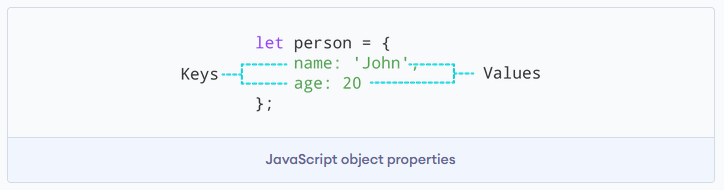
\includegraphics[width=\textwidth]{images/JavaScript_Object.PNG}
\caption[JavaScript Objekt]{JavaScript Objekt \cite{JS1.29}}
\label{fig:JavascriptObjekt}
\end{figure}

\subsubsection{Anwendungsgebiete}
Ursprünglich fand JavaScript seinen Einsatz hauptsächlich darin, dynamische Webseiten im Web\-browser anzuzeigen. Die Verarbeitung erfolgte dabei meist clientseitig durch den Webbrowser (dem sogenannten Frontend) \cite{JS1.3}.
\newline
\noindent
Heutzutage findet sich die Sprache dagegen in wesentlich größeren Einsatzgebieten wieder. 
Bis vor einigen Jahren war die Serverseite anderen Programmiersprachen wie Java oder PHP vorbehalten. Die Veröffentlichung von Node.js, einer plattformübergreifenden Laufzeitumgebung, die JavaScript außerhalb eines Webbrowsers ausführen kann, führte zu einer immer größeren Verbreitung von serverseitigen Anwendungen (dem Backend), die auf JavaScript basieren. Auf Node.js wird ausführlicher im nächsten Kapitel eingegangen. 
Ferner findet JavaScript heutzutage aber auch seinen Einsatz in mobilen Anwendungen, Desktopanwendungen, Spielen oder 3D-Anwendungen \cite{JS1.4}.

